\documentclass[12pt]{article}
\DeclareMathSizes{12}{13}{10.4}{10.4}
\usepackage[utf8]{inputenc}
\usepackage[margin=1.5cm]{geometry}
\usepackage{amsmath}
\usepackage{amssymb}
\usepackage{cancel}
\usepackage{graphicx}

\begin{document}
\section*{LEZIONE 8: INTRODUZIONE ALLA SOLUZIONE NUMERICA DI EQUAZIONI NON LINEARI, METODO DI BISEZIONE}
In questa e nelle prossime 3 lezioni ci occupiamo di un argomento classico del calcolo numerico, ovvero la soluzione numerica (cioè approssimata) di equazioni non lineari. Tratteremo 2 tipi di equazioni
\begin{itemize}
    \item $f(x)=0$, zeri di funzione
    \item $x=\phi(x)$, equazioni di punto fisso
\end{itemize}
che possiamo schematizzare coi seguenti disegni
\begin{center}
        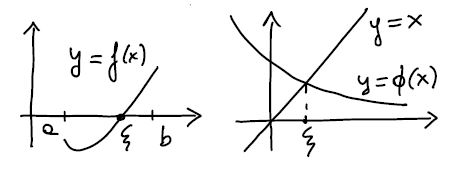
\includegraphics[width=0.5\textwidth]{1.JPG}\par
\end{center}
Il primo tipo corrisponde al calcolo di uno zero di una funzione (continua), cioè di un punto $\xi$ in cui $f$ si annulla. Il secondo tipo corrisponde invece al calcolo del punto fisso $\xi$ di una funzione (continua) $\phi$ e si può interpretare come calcolo dell'ascissa dell'intersezione del grafico della bisettrice del primo e terzo quadrante y=x col grafico di $y=\phi(x)$.\\ In entrambi i casi daremo \underline{condizioni sufficienti} per \underline{l'esistenza} ($\exists$) e l'unicità (!) della soluzione in un dato intervallo e discuteremo, analizzando in dettaglio, tre metodi classici di soluzione: i metodi di \underline{BISEZIONE} e di \underline{NEWTON} (tangenti) per gli zeri e il metodo delle \underline{ITERAZIONI DI PUNTO FISSO}.\\
Cominciamo col ricordare alcuni risultati di esistenza e unicità nel caso della ricerca di zeri.\\ \underline{TEOREMA} (degli zeri di funzioni continue)\\
Sia $f(x)\in C[a,b]$ (cioè f continua nell'intervallo chiuso e limitato [a,b] e $f(a)f(b)<0$ cioè f cambia segno agli estremi) $\Rightarrow \exists$ $ \xi\in(a,b):f(\xi)=0$\\ Osserviamo che tale zero può non essere unico:
\begin{center}
        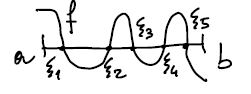
\includegraphics[width=0.3\textwidth]{2.JPG}\par
\end{center}
D'altra parte togliendo una delle ipotesi la condizione restante \underline{non} basta a garantire l'$\exists$
\begin{center}
        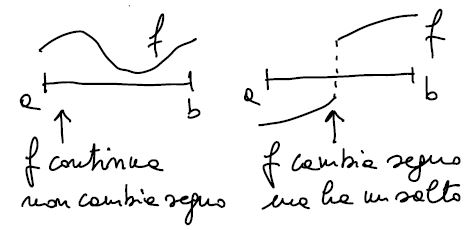
\includegraphics[width=0.5\textwidth]{3.JPG}\par
\end{center}
Ribadiamo che le condizioni \underline{non} sono \underline{necessarie}
\begin{center}
            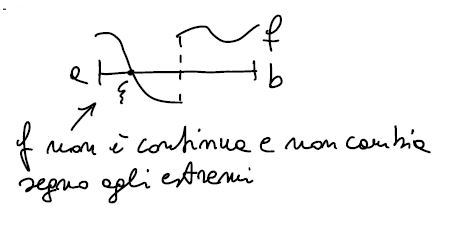
\includegraphics[width=0.5\textwidth]{4.JPG}\par
\end{center}
diamo anche due classiche condizioni \underline{sufficienti} ciascuna delle quali garantisce l'\underline{unicità} dello zero
\begin{itemize}
    \item $f$ \underline{strettamente monotona} (strettamente crescente o decrescente in $[a,b]$
    \item $f \in C[a,b]$, $f(a)f(b)<0$ e $f$ \underline{strettamente convessa} o \underline{concava} in $[a,b]$
\end{itemize}
Nel caso in cui $f$ è derivabile in $[a,b]$ la monotonia stretta è legata al segno di $f'$

\begin{equation*}
    f'(x)>0 \ in \ [a,b] \Rightarrow f \ strettamente \ crescente
\end{equation*}
\begin{equation*}
    f'(x)<0 \ in \ [a,b] \Rightarrow f \ strettamente \ decrescente
\end{equation*}
Ricordiamo che il viceversa è vero
Con la diseguaglianza non stretta,
\begin{equation*}
    f \ strettamente \ crescente \Rightarrow f'(x)\geq0 \ in \ [a,b] 
\end{equation*}
\begin{equation*}
    f \ strettamente \ decrescente \Rightarrow f'(x)\leq0 \ in \ [a,b] 
\end{equation*}
come si vede ad esempio con la funzione $f(x)=x^3$ in $[-1,1]$
\begin{center}
            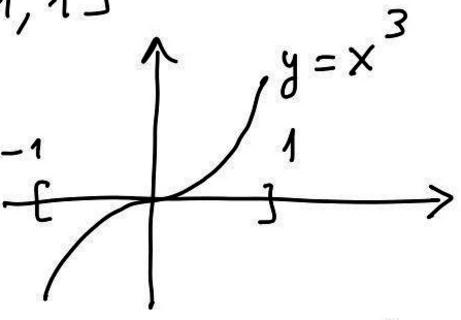
\includegraphics[width=0.3\textwidth]{5.jpg}\par
\end{center}
Per cui si ha che $f$ è strettamente crescente ma $f'(0)=3x^2|_{x=0}=0$.\\
\smallskip
Analogamente convessità e concavità stretta sono legate al segno di $f''$ quando $f$ è derivabile 2 volte in $[a,b]$\\
\begin{center}
    $f''(x) > 0 $ in $[a,b] \Rightarrow f$ strettamente conv.\\
\end{center}
\begin{center}
    $f''(x) < 0 $ in $[a,b] \Rightarrow f$ strettamente conc.\\
\end{center}
Di nuovo, il viceversa è vero con la disuguaglianza non stretta
\begin{center}
    $f$ strettamente conv. $\Rightarrow f''(x) \geq 0 $ in $[a,b]$
\end{center}
\begin{center}
   $ f $ strettamente conc. $ \Rightarrow f''(x) \leq 0 $ in $[a,b]$
\end{center}
\begin{center}
    ($f(x) = x^4$ è  strettamente conv. in $[-1,1]$, $f''(0) = 0$)
\end{center}
Ribadiamo che le condizioni di unicità date sono solo sufficienti 
\begin{center}
            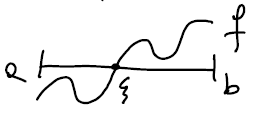
\includegraphics[width=0.3\textwidth]{pagina8_1.png}\par
\end{center}
\begin{center}
non è ne monotona ne convessa o concava ma $\xi$ è unico\\
\end{center}
Fatti questi brevi richiami teorici su $\exists!$ delle soluzioni di equazioni scritte nella forma $f(x)=0$, $x \in [a,b]$, introduciamo uno dei metodi più semplici per la soluzione numerica, il \textbf{metodo} \textbf{di} \textbf{bisezione}.

\subsubsection*{METODO DI BISEZIONE}
Il metodo di bisezione consiste nell'applicazione iterativa del teorema degli zeri di funzioni continue, quindi si assume che $f \in C[a,b]$, $f(a)f(b)<0$. \\
Illustriamo graficamente la costruzione delle iterazioni
\begin{center}
            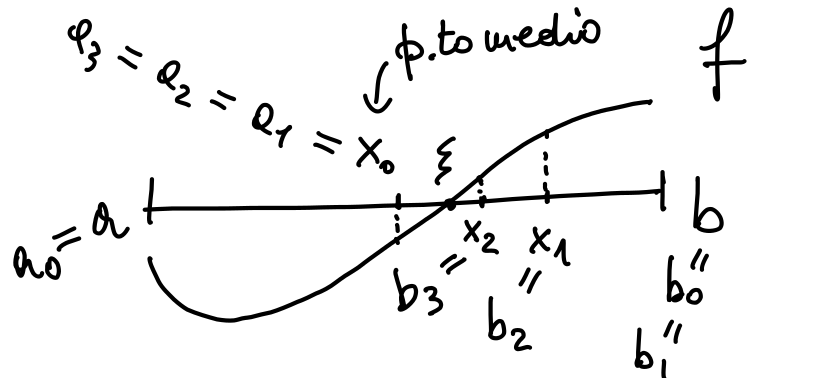
\includegraphics[width=0.5\textwidth]{im_pag10.png}\par
\end{center}
L'idea è la seguente: si parte da $[a_0,b_0]=[a,b]$, si calcola il punto medio $x_0=\frac{(a_0+b_0)}{2}$; ora se $f(x_0)=0$ siamo su uno zero; altrimenti siccome $f(a_0)$ e $f(b_0)$ hanno segno definito, $f(x_0)$ sarà discorde con uno solo dei due e quindi sicuramente ci sarà uno zero in $(a_0,x_0)$ se $f(a_0)f(x_0)<0$ altrimenti ci sarà uno zero in $(x_0, b_0)$ visto che $f(x_0)f(b_0)<0$ (sempre per il teorema degli zeri). Nel primo caso si definisce $a_1=a_0$, $b_1=x_0$, mentre nel secondo $a_1=x_0$, $b_1=b_0$, con la garanzia che $\exists \ \xi \in (a_1,b_1)$ tale che $f(\xi)=0$ visto che $f(a_1)f(b_1)<0$.\\
Il procedimento viene iterato applicando ripetutamente il teorema degli zeri per passare da $[a_n,b_n]$ ad $[a_{n+1},b_{n+1}]$ in cui uno degli estremi è diventato il punto medio $x_n=\frac{(a_n+b_n)}{2}$ di $[a_n,b_n]$.\\
Si tratta in generale di un processo infinito (a meno che per qualche $n$ non risulti $f(x_n)=0$) che permette di costruire 3 successioni ${ a_n } , { b_n } , { x_n } $ tali che:
\begin{itemize}
    \item $\exists \xi : f(\xi)=0, \ \xi \in (a_n,b_n)$
    \item $|\xi - a_n|, \ |\xi - b_n| \leq b_n-a_n=\frac{b-a}{2^n}$
    \item $|\xi - x_n| < \frac{b_n - a_n}{2} = \frac{b-a}{2^{n+1}}$
\end{itemize}
$n=0,1,2,\dots$ \\
Il nome "bisezione" viene dal fatto che l'intervallo viene diviso iterativamente a metà, "buttando via" ad ogni iterazione mezzo intervallo per restare nella metà dove $f$ cambia segno e dove quindi c'è sicuramente uno zero ("lo" zero nel caso questo sia unico in $(a,b)$, ma in generale il metodo funziona anche con vari zeri, calcolandone uno). Si vede subito che il metodo è convergente, cioè che tutte e 3 le successioni convergono ad uno zero $\xi \in (a,b)$
Infatti
\begin{equation*}
    0 \leq |\xi - a_n|, \ |\xi - b_n| < \frac{b-a}{\underbrace{2^n}_{\rightarrow \infty}} \longrightarrow 0
\end{equation*}
e per il teorema dei 2 carabinieri
\begin{equation*}
    |\xi - a_n|, \ |\xi - b_n| \longrightarrow 0, \ n \rightarrow \infty
\end{equation*}
analogamente
\begin{equation*}
    |\xi - x_n| \longrightarrow 0, \ n \rightarrow \infty
\end{equation*}
visto che $0 \leq |\xi - x_n| < \frac{b-a}{2^{n+1}}$.\\
Quest'ultima diseguaglianza è immediatamente comprensibile da questo disegno
\begin{center}
            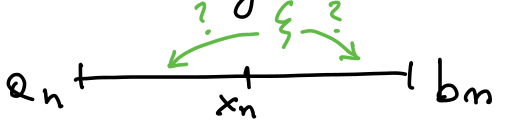
\includegraphics[width=0.5\textwidth]{6.png}\par
\end{center}
Cioè sappiamo che $\xi$ zero di $f$ sta in $(a_n, b_n)$, non sappiamo dove, ma sicuramente la sua distanza dal punto medio $x_n$ è minore di metà della lunghezza dell'intervallo $[a_n, b_n]$ cioè è $\frac{(b_n - a_n)}{2}$, in altri termini, $\xi$ sta nell'intorno aperto di centro $x_n$ e raggio $\frac{(b_n - a_n)}{2}$. Nel metodo di bisezione si sceglie $x_n$ come successione di approssimazioni, visto che la \underline{stima} dell'errore è migliore di un fattore $\frac{1}{2}$ rispetto a quella di $a_n$ e $b_n$. Volendo garantire una tolleranza di $\varepsilon > 0 $ nel calcolo approssimato del vero $\xi$, basta quindi risolvere la disuguaglianza di 
\begin{equation*}
    e_n = | \xi - x_n | < \frac{b-a}{2^{2n+1}} \leq \varepsilon
\end{equation*}
in modo che $\xi \in (x_n -  \varepsilon, x_n + \varepsilon)$, ovvero 
\begin{equation*}
    2^{n+1} \geq  \frac{b-a}{\varepsilon}
\end{equation*}
cioè
\begin{center}
   $n + 1 \geq \log_2{\frac{b-a}{\varepsilon}}$
\end{center}
\begin{center}%Da mettere il numero in questa ? 
    $ = log_2{(b-a)} + log_2(\frac{1}{\varepsilon})$
\end{center}
Questa disuguaglianza permette "a priori", cioè prima di iniziare il processo di calcolo, di decidere a quale iterazione fermarsi in modo da garantire la tolleranza di $\varepsilon > 0$, basta prendere 
\begin{center} %Da mettere il numero in questa ? 
    $n(\varepsilon) = [\log_2(\frac{1}{\varepsilon}) + log_2{(b-a)}]$
\end{center}
in effetti una stima del tipo $e_n \leq stima(n)$ dove la stima non dipende dalle quantità calcolate si chiama usualmente "STIMA A PRIORI"
\\Il problema con le stime a priori è che sono spesso SOVRASTIME, cioè non sono vicine all'errore effettivo ma ne danno solo un confine superiore garantito in modo teorico, che però può portare a un aumento del numero di iterazioni e quindi del costo computazionale, rispetto a quello che sarebbe sufficiente ad ottenere la tolleranza richiesta.
Per ottenere una stima dell'errore piú aderente, cominciamo col fare la seguente osservazione: visto che $x_n \to \xi,\,n\to \infty$ e che $f$ è continua, si avrà che \[f(x_n) \to f(\xi)=0,\quad n \to \infty\]
Quella che stiamo usando qui in realtà è una caratterizzazione della continuità di una funzione in analisi matematica: $f$ è continua in $l$ \underline{se e solo se}
\[\forall \{x_n\}:\lim_{n\to \infty}x_n=l \text{ si ha } \lim_{n\to \infty}f(x_n)=f(l)\]
che si esprime anche dicendo "$f$ è continua se e solo se il limite si può trasportare 'dentro' la funzione".\\
Nel nostro caso $f(\xi)=0$ quindi $f(x_n) \to 0,\,n \to \infty$ e anche $|f(x_n)|\to 0,\,n \to \infty$.\\
La quantità $|f(x_n)|$ si chiama "RESIDUO" perchè dice quanto "resta" ad $f$ per annullarsi.\\
Viene allora spontanea questa domanda: siccome $f(x_n) \to 0,\,n \to \infty$, possiamo arrestare il processo di calcolo quando il residuo $|f(x_n)|$ è piccolo? In altre parole
\[|f(x_n)|\le \varepsilon \overset{?}{\Longrightarrow} e_n \le \varepsilon\]
\\la risposta è \underline{NO}, in realtà\\
\begin{center}
$\left| f(x_n)\right|\le \varepsilon \nRightarrow e_n\le \varepsilon$
\end{center}
perchè come vedremo subito la grandezza del residuo non è in se' un buon indicatore dell'errore, ma va opportunamente "pesata": per capirlo consideriamo i seguenti grafici\\
\begin{center}
    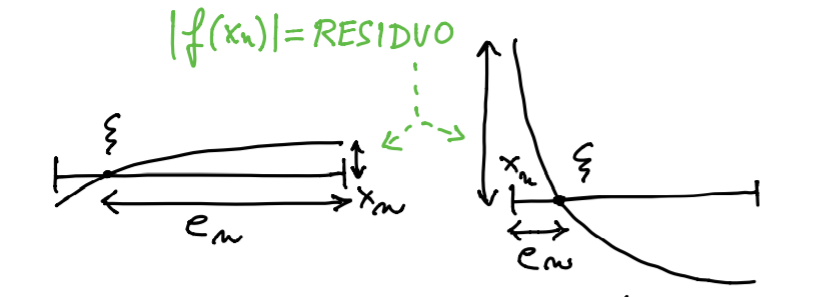
\includegraphics[width=0.6\textwidth]{grafo4.png}
\end{center}
nel primo caso il residuo è piccolo ma l'errore è grande (cioè il residuo è una \underline{SOTTOSTIMA} dell'errore).
\\Nel secondo caso il residuo è grande ma l'errore è piccolo (cioè il residuo è una \underline{SOVRASTIMA} dell'errore).\\
È importante osservare che una \underline{sottostima} dell'errore in pratica è la cosa piú \underline{pericolosa}, perchè induce a fermare le iterazioni quando $x_{n}$ non è ancora nell'intorno del limite individuato dalla tolleranza: si pensa di aver approssimato la quantitá limite a meno della tolleranza e invece \underline{l'errore è piú grande della tolleranza}.
\\Questo può chiaramente portare a conseguenze gravi in applicazioni in cui il rispetto della tolleranza è decisivo.
D'altra parte, una \underline{sovrastima} pur essendo meno grave, ha come conseguenza un aumento del numero di iterazioni rispetto a quello che sarebbe sufficiente e quindi un \underline{incremento} del \underline{costo computazionale}.\\
Nei due grafici disegnati sopra si nota che il residuo è una sottostima dell'errore quando la funzione è "piatta", cioè la variazione è lenta in un intorno dello zero, mentre è una sovrastima quando la funzione è "ripida", cioè ha una variazione veloce in un intorno dello zero.
Si capisce allora che il residuo va in qualche modo "pesato" per tener conto della velocitá di variazione: se $f$ è derivabile, bisogna quindi tenere conto della grandezza della derivata, che per definizione misura la velocitá di variazione di una funzione per fare questo in modo rigoroso possiamo ricorrere a un teorema chiave del calcolo differenziale, il teorema del VALOR MEDIO (detto anche teorema di Lagrange).\\\\
\underline{TEOREMA} (del valor medio)\\
Sia $f \in C[\alpha,\beta]$ derivabile in $(\alpha,\beta) \Longrightarrow \exists\, z\in (\alpha,\beta)$ tale che \[\frac{f(\beta) - f(\alpha)}{\beta - \alpha} = f'(z)\] \newline
Interpretazione geometrica
\begin{center}
   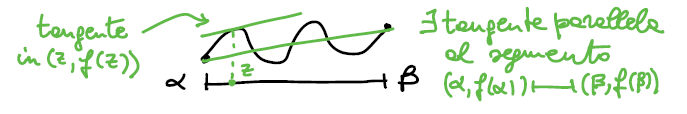
\includegraphics{pag25} 
\end{center}
Tornando all'analisi del residuo nel metodo di bisezione, mettiamoci nelle seguenti ipotesi: $f\in C^1[a,b]$ (cioè $f$ è derivabile con derivata prima continua in $[a,b]$), $\{x_n\}\subset[c,d]\subseteq[a,b]$ (almeno per $n\ge n_0$ cioè per $n$ abbastanza grande) con \[x_n \to \xi,\,n \to \infty,\,f(\xi)=0 \text{ e } f'(x)\ne 0\quad \forall x\in [c,d]\] allora vale la rappresentazione:
\[e_n=|x_n-\xi|=\frac{|f(x_n)|}{|f'(z_n)|},\quad n\ge n_0\] con $z_n\in int(x_n,\xi)$, l'intervallo aperto che ha per estremi $x_n$ e $\xi$ (potrebbe essere $(x_n,\xi)$ oppure $(\xi,x_n)$ a seconda che $x_n<\xi$ oppure $x_n>\xi$).\\
Prima di dimostrare la stima, osserviamo che
\begin{enumerate}
    \item la rappresentazione dell'errore mostra chiaramente che l'\underline{ERRORE} è un \underline{RESIDUO PESATO} della derivata;
    \item l'ipotesi che $f'(x)\ne0$ in $[c,d]\subseteq [a,b]$ è equivalente all'ipotesi che lo zero sia SEMPLICE, ovvero che $f'(\xi)\ne 0$ (la terminologia viene dalle equazioni algebriche, cioè quelle in cui $f$ è un polinomio, lì zero semplice significa che $(x-\xi)^{\alpha}$ compare con $\alpha =1$ nella fattorizzazione di Ruffini). Infatti, se $x_n\in [c,d]\quad \forall n>n_0$ allora $\xi=\lim x_n\in [c,d]$ perchè $[c,d]$ è chiuso e quindi contiene i limiti delle successioni lì contenute, quindi $f'(\xi)\ne 0$.
    Viceversa, se $f'(\xi)\ne 0$ siccome $f'$ è continua, per il teorema della \underline{permanenza del segno}
    \[\exists\, \delta>0 : f'(x)\ne 0\quad \forall x \in [\xi - \delta, \xi + \delta] = [c,d]\]
    e siccome $x_n \to \xi,\,n \to \infty\quad \exists \,n_0$ tale che $|x_n-\xi|\le \delta \quad \forall n \ge n_0$\\
    Si noti che $f'(z_n)\ne 0,\, n\ge n_0$ perchè $z_n \in int(x_n,\xi)\subset[c,d]$.\\
    È importante osservare che la rappresentazione dell'errore come residuo pesato non vale solo per il metodo di bisezione, ma per ogni metodo convergente a uno zero semplice se $f\in C^1$ (applicheremo infatti questo risultato più avanti al metodo di Newton)
    \item dalla rappresentazione siamo in grado di ricavare delle STIME A POSTERIORI dell'errore (a posteriori perchè si utilizza il residuo che è calcolabile solo a posteriori dopo aver prodotto $x_n$ nel processo di calcolo)
\end{enumerate}
    \underline{DIMOSTRAZIONE} della rappresentazione utilizzando il teorema del valor medio e supponendo che $x_n>\xi$ (l'altro caso è del tutto analogo), con $\alpha=\xi, \beta=x_n$
\begin{equation*}
	f(x_n)-f(\xi) = f'(z_n)(x_n-\xi), \text{ } z_n \in (\xi,x_n)
\end{equation*}
con $f(\xi)=0$, cioè
\begin{equation*}
	|f(x_n)| = |f'(z_n)||x_n-\xi|
\end{equation*}
che si può riscrivere come
\begin{equation*}
	e_n = |x_n-\xi| = \frac{|f(x_n)|}{|f'(z_n)|}
\end{equation*}

Ora, siccome il teorema del valor medio non dice chi sia $z_n$ ma solo che esiste almeno un $z_n$ in $int(x_n,\xi)$, cerchiamo di ricavare delle stime "pratiche" dell'errore utilizzando il residuo opportunamente pesato.
\\
i) Se è noto che $|f'(x)| \geqslant k >0$ $\forall x \in [a,b]$ (ma basta $\forall x \in [c,d]$), allora
\begin{equation*}
	e_n = \frac{|f(x_n)|}{f'(z_n)} \leqslant \frac{|f(x_n)|}{k}
\end{equation*} 
ii) Se $f'$ è nota o calcolabile, siccome $z_n \to \xi, n \to \infty$ per il teorema dei 2 carabinieri visto che $z_n$ sta fra $\xi$ e $x_n$, per la continuità di $f'$ si ha che
\begin{equation*}
	|f'(x_n)|, \text{ } |f'(z_n)| \to |f'(\xi)| \neq 0, \text{ per } n \to \infty
\end{equation*}
Quindi, almeno per $n$ abbastanza grande, $|f'(x_n)|$ e $|f'(z_n)|$  saranno entrambi dell'ordine di grandezza di $|f'(\xi)|$ (notiamo che nel residuo pesato quello che interessa è essenzialmente \underline{l'ordine di} \underline{grandezza del peso} $|f'(z_n)|$: per fissare le idee, sto dividendo per $100$ o per $\frac{1}{100}$? Cioè, sto "aggiustando" una sovrastima o una sottostima?).\\
Abbiamo quindi una "STIMA EMPIRICA":
\begin{equation*}
	e_n = |x_n-\xi| \approx \frac{|f(x_n)|}{|f'(x_n)|}
\end{equation*} 
valida almeno per $n \geqslant \bar{n}$, dove $\bar{n}$ corrisponde ad un controllo empirico che l'ordine di grandezza di $|f'(x_n)|$ si stia "stabilizzando", cioè valga:
\begin{equation*}
	\lvert\frac{|f'(x_n)|}{|f'(x_{n-1})|}-1\rvert \leqslant \delta
\end{equation*} 
Ad esempio con $\delta = 10^{-1}$ o $10^{-2}$ $\frac{|f'(x_n)|}{|f'(x_{n-1})|} \to 1$, $n \to \infty$, quindi ha senso controllare quando il rapporto si sta stabilizzando intorno a $1$, tenendo presente che questo è un criterio sensato ma non completamente rigoroso, diciamo una "linea guida" per l'utilizzo del peso \\ 
iii) Se $f'$ non è vuota esplicitamente, va in qualche modo approssimata.\\Osserviamo infatti che non sempre abbiamo a disposizione una formula analitica per $f$ (come ad es. per l'equazione algebrica $x^2-2=0$ corrispondente al calcolo di $\sqrt{2}$ o per l'equazione non algebrica $x-e^{-x}=0$)\\Infatti $f$ potrebbe essere nota in forma di "scatola nera"\\
\begin{center}
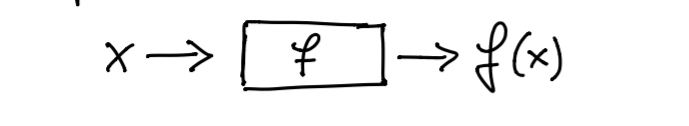
\includegraphics[width=0.4\textwidth]{scatolanera.PNG}    
\end{center}
cioè potremmo avere a disposizione solo i valori da misure o da altri algoritmi. Se però sappiamo almeno che $f$ è derivabile, possiamo approssimare $f'$ con un rapporto incrementale costruito con le quantità calcolate \\ 
\[f'(z_n)\approx \vartheta_n=\frac{f(x_n)-f(x_{n-1})}{x_n-x_{n-1}}\overset{\overset{\text{\tiny{ VALOR \ MEDIO}} }{\downarrow}}{=} f'(\mu_n)\]
dove $int(x_n,x_{n-1})\ni \mu_n \rightarrow \xi, n\rightarrow\infty$ e quindi 
\[|\vartheta_n|\approx|f'(\xi)|\approx|f'(z_n)|\] almeno per $n$ abbastanza grande: di nuovo, possiamo usare un criterio empirico per "accettare" il valore di $|\vartheta_n|$ come peso, tipo $|\frac{|\vartheta_n|}{|\vartheta_{n-1}|}-1|\leq \delta$ \\
detto $k_n$ il peso calcolato con uno degli approcci $(i)-(iii)$, siamo allora in grado di scrivere un "$\underline{test \  di \  arresto}$" per il metodo di bisezione che $\underline{combina}$ stima $\underline{a \  priori}$ e stima $\underline{a \  posteriori}$\\
$min\{\frac{b-a}{2^{n+1}},\frac{|f(x_n|}{k_n}\}\leq \varepsilon$
\\Possiamo a questo punto fare alcune considerazioni di carattere computazionale.\\
A) il metodo di bisezione funziona con $\underline{richieste}$ analitiche e computazionali $\underline{minime}$.
La versione base con la stima a priori chiede solo che siano soddisfatte le ipotesi del teorema degli zeri (continuità e cambio segno agli estremi) e unicamente la possibilità di calcolare correttamente il segno di $f(x_n)$ (per cui è sufficiente un errore relativo $<100\%$ su $f(x_n)!$)
infatti in generale se $\tilde{\alpha} \approx \alpha \neq 0$ e $\frac{|\alpha-\tilde{\alpha}|}{|\alpha|}<1 \Rightarrow sgn(\tilde{\alpha})=sgn(\alpha)$\\
B) mentre la stima a priori è decrescente, l'errore effettivo in generale non lo è, come si vede da questo disegno
\begin{center}
    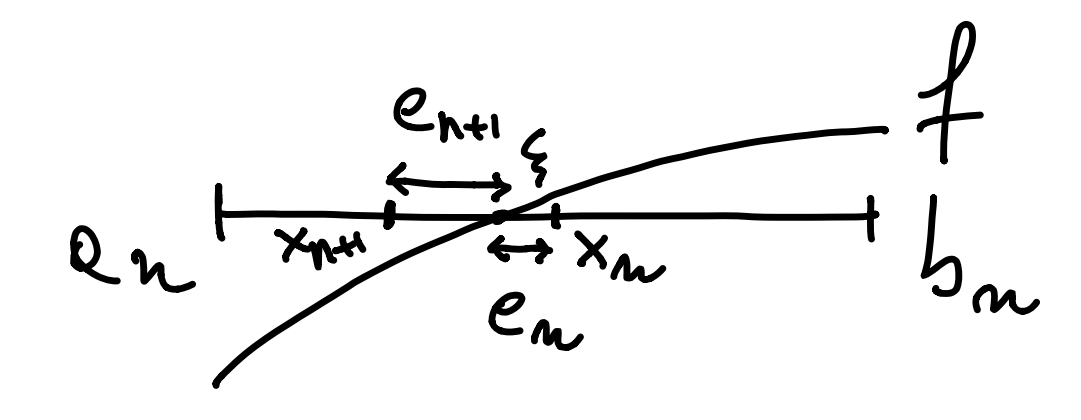
\includegraphics[width=0.4\textwidth]{grafo3.png}\par
\end{center}
 dove $e_{n+1}>e_n$ ( anche se comunque $e_n \rightarrow 0, n \rightarrow \infty$); qui si vede anche che $e_n\ll\frac{(b_n-a_n)}{2}$ e la stima del residuo pesato è tendenzialmente più accurata a differenza della stima a priori che si dimezza, $e_{n+1}\approx\frac{e_n}{2}$ solo "in media" su un po' di iterazioni.\\
Concludiamo la lezione con un esempio, il calcolo approssimato di $\sqrt{2}$ risolvendo l'equazione algebrica $x^2 -2 = 0$ con il metodo di bisezione.\\
\underline{ESEMPIO: }(calcolo di $\sqrt{2}$ alla precisione di macchina)\\ Consideriamo l'equazione algebrica
\[f(x)=x^2-2=0\] Calcolarne la soluzione positiva significa calcolare $\sqrt{2}$. Le ipotesi del teorema degli zeri sono soddisfatte in $[a,b]=[1,2]$.\\
Infatti $f\in C[a,b]$ (anzi $f\in C^{\infty}(\mathbb{R})$ cioè è derivabile infinite volte in $\mathbb{R}$ con derivate tutte continue, perché $f$ è un polinomio) \[f(a)=f(1)=1-2=-1<0\] \[f(b)=f(2)=2^2-2=2>0\]
Inoltre $f'(x)=2x \geq 2\quad\forall x \in [1,2]$ quindi $\sqrt{2}\in (1,2)$ ed è l'unico zero in tale intervallo (in effetti sappiamo che è l'unico zero in $\mathbb{R}^+$)
possiamo applicare il metodo di bisezione che comincia in questo modo: $x_0=\frac{1+2}{2}=1.5$, $x_1=\frac{1+1.5}{2}=1.25$, $x_2=\frac{1.25+1.5}{2}=\frac{2.75}{2}=1.375$,  $x_3=\frac{1.375+1.5}{2}=1.4375$, \dots (ricordiamo che $\sqrt{2}=1.4142\dots$).\\
Nel grafico sottostante (in scala log) riportiamo l'errore effettivo, la stima a priori \[\frac{(b_n-a_n)}{2}=\frac{1}{2^{n+1}}\] 
e la stima a posteriori \[\frac{|f(x_n)|}{k}=\frac{|x_n^2-2|}{2}\]
(visto che $f'(x)\ge k=2 \quad \forall x\in [1,2]$) tutte relativizzate a $|\xi|=\sqrt{2}$ (in questo caso comunque $|\xi|$ è dell'ordine dell'unità e quindi errore assoluto e relativo vicini) \\
\begin{center}
    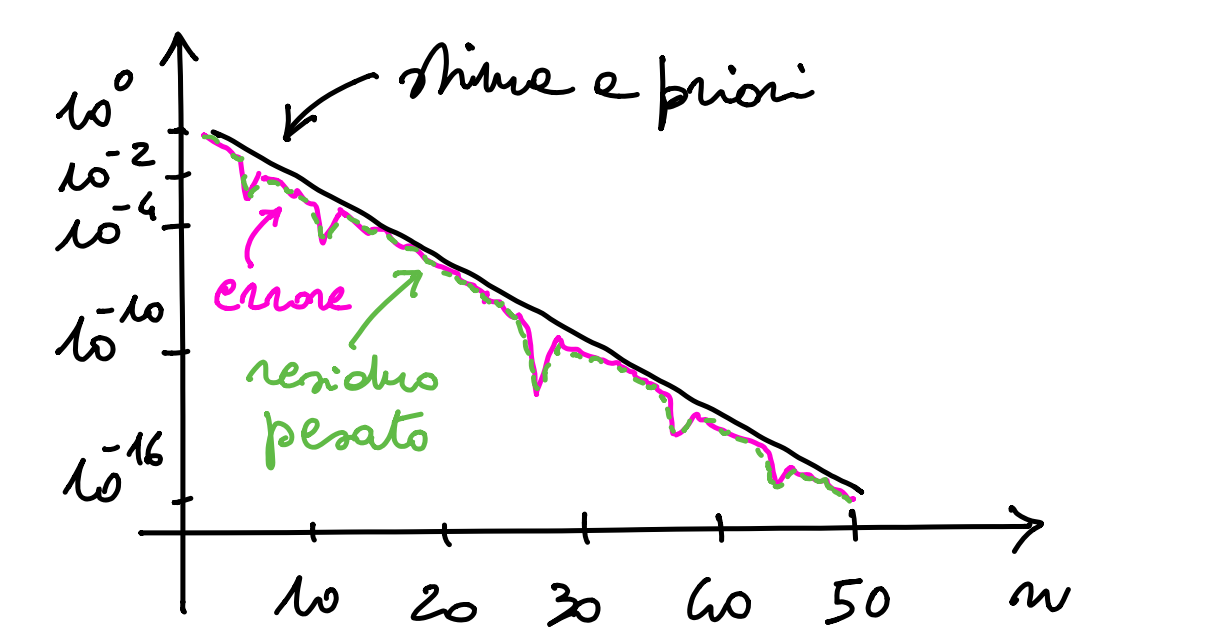
\includegraphics[width=0.5\textwidth]{grafo2.png}\par
\end{center}
(come sempre per comodità i valori discreti sono interpolati con linee continue o tratteggiate).\\
Si vede che l'errore segue solo "in media" l'andamento della stima a priori, che la sovrastima a volte di vari ordini di grandezza (picchi dell'errore verso il basso, ad esempio tra $n=20$ e $n=30$ l'errore va circa a $10^{-11}$ mentre la stima a priori ha bisogno di una decina di iterazioni in più).\\
D'altra parte la stima del residuo pesato è praticamente sovrapposta all'errore effettivo.\\
Si noti infine che per raggiungere un errore dell'ordine della precisione di macchina $\epsilon_M=2^{-53}$ servono circa $50$ iterazioni, il che non è sorprendente visto che il fattore medio di riduzione dell'errore è $\frac{1}{2}$.
\end{document}
